\chapter{Mecânica Não-Linear}\label{ch:MecNlgeo}
\section{Introdução}
Até agora, assumimos que os deslocamentos são pequenos o suficiente para considerar que a sua relação com a deformação é linear. Também assumimos que o material responde da mesma maneira em qualquer estado de carregamento (material Linear) e que se retirarmos a carda do corpo, seu estado deformado volta exatamente ao estado anterior indeformado (material em regime elástico). Com essas hipóteses, podemos chegar no problema linear que tem como incógnita o campo de deslocamento do domínio $\Omega$

\begin{equation}
	\mathbf{K} \mathbf{u} = \mathbf{F},
\end{equation}

fatores como o nível de carga, geometria e comportamento do material podem facilmente causar diferenças consideráveis entre os resultados das equações lineares e o fenômeno real. O que causa essa diferença são os grandes deslocamentos que invalida a hipótese linear que a porção com termos quadráticos na equação de deformação podia ser desconsiderada

\section{Princípio da Mínima Energia Potencial}
A forma fraca de um sistema elástico não linear pode ser derivada do princípio da energia potencial mínima. A energia potencial de um sistema elástico é a diferença entre a energia de deformação armazenada $\Pi_{\text{int}}$ e o trabalho realizado pelas forças externas $\Pi_{\text{ext}}$. A energia de deformação pode ser obtida integrando a função de densidade de energia de deformação na Eq.~\eqref{eq:DensidadeEnergia} sobre a geometria inicial indeformada. O trabalho realizado pelas forças aplicadas é calculado multiplicando o deslocamento pelas forças aplicadas.

A energia potencial $\Pi(u)$ de um sistema elástico é dada por:
\begin{equation}\label{eq:PMEP}
	\Pi(u) = \Pi_{\text{int}}(u) - \Pi_{\text{ext}}(u) = \iint_{\Omega_0} W(\mathbf{E}) , d\Omega - \iint_{\Omega_0} \mathbf{u}^T \mathbf{f}_b , d\Omega - \int_{\Gamma_s} \mathbf{u}^T \mathbf{t} , d\Gamma,
\end{equation}
onde $\mathbf{f}_b$ é a força de corpo, $\mathbf{t}$ é a força de tração superficial na fronteira $\Gamma_s$, e $\mathbf{E}$ é a deformação Lagrangiana, definida como:
\begin{equation}
	\mathbf{E} = \frac{1}{2}\left(\mathbf{F}^T\mathbf{F}-\mathbf{I}\right)=\frac{1}{2} \left( \nabla_0 \mathbf{u} + \nabla_0 \mathbf{u}^T + \nabla_0 \mathbf{u} \nabla_0 \mathbf{u}^T \right),
\end{equation}
onde $\nabla_0$ é o operador gradiente na geometria não deformada.

O princípio da energia potencial mínima afirma que o campo de deslocamento $\mathbf{u} \in \mathbbm{V}$ em equilíbrio minimiza a Eq.~\eqref{eq:PMEP}. 

Para encontrar este deslocamento de equilíbrio, aplica-se um método de perturbação. Assume-se que o campo de deslocamento $\mathbf{u}$ é perturbado na direção de um deslocamento arbitrário $\mathbf{\bar{u}}$ com $\tau$ como parâmetro controlando o tamanho da perturbação. O deslocamento perturbado $\mathbf{u}_\tau$ é então:
\begin{equation}
	\mathbf{u}_\tau = \mathbf{u} + \tau \mathbf{\bar{u}}.
\end{equation}

Note que $\mathbf{\bar{u}}$ corresponde ao deslocamento virtual no princípio do trabalho virtual. Nesta equação, a solução perturbada $u_\tau$ também pertence ao espaço de solução $\mathbbm{V}$. Consequentemente, a variação $\mathbf{\bar{u}}$ deve satisfazer a condição de contorno essencial homogênea, ou seja, $u \in \mathbbm{Z}$.

A primeira variação da energia potencial é obtida tomando a variação de primeira ordem de $\Pi(\mathbf{u})$ na direção de $\mathbf{\bar{u}}$:
\begin{equation}\label{eq:derivPi}
	\bar{\Pi}(\mathbf{u}, \mathbf{\bar{u}}) = \frac{d}{d\tau} \Pi(\mathbf{u} + \tau \mathbf{\bar{u}}) \Big|_{\tau=0},
\end{equation}
onde o símbolo de barra representa a variação de primeira ordem de uma função. $\Pi(\mathbf{u})$ depende apenas de $\mathbf{u}$, enquanto $\bar{\Pi}(\mathbf{u}, \mathbf{\bar{u}})$ depende tanto de $\mathbf{u}$ quanto de sua variação $\mathbf{\bar{u}}$. Usando a energia potencial na Eq.~\eqref{eq:PMEP} e igualando a primeira variação a zero, obtém-se a seguinte equação variacional:
\begin{equation}\label{eq:derivPMEP}
	\bar{\Pi}(\mathbf{u}, \mathbf{\bar{u}}) = \iint_{\Omega_0} \frac{\partial W(\mathbf{E})}{\partial \mathbf{E}} : \mathbf{\bar{E}} d\Omega - \iint_{\Omega_0} \mathbf{u}^T \mathbf{f}_b , d\Omega - \int_{\Gamma_s} \mathbf{u}^T \mathbf{t} , d\Gamma = 0.
\end{equation}
Na equação acima, a variação do trabalho realizado pelas cargas aplicadas é direta, pois é linear em relação ao deslocamento $\mathbf{u}$. A variação da densidade de energia de deformação, tomada em relação à deformação Lagrangiana usando a regra da cadeia, dá:
\begin{equation}
	\begin{split}
		\mathbf{\bar{E}}(\mathbf{u}, \mathbf{\bar{u}}) = \frac{d}{d\tau} \mathbf{E}(\mathbf{u} + \tau \mathbf{\bar{u}}) \Big|_{\tau=0} &= \frac{1}{2} \left( \nabla_0 \mathbf{\bar{u}}^T + \nabla_0 \mathbf{\bar{u}} + \nabla_0 \mathbf{\bar{u}}^T \nabla_0 \mathbf{u}  + \nabla_0 \mathbf{u}^T \nabla_0 \mathbf{\bar{u}} \right) \\
		& =\text{sym}\left(\nabla_0\mathbf{\bar{u}}^T+ \nabla_0 \mathbf{\bar{u}}^T \nabla_0 \mathbf{u}\right)\\
		& =\text{sym}\left(\nabla_0\mathbf{\bar{u}}^T\mathbf{F}\right),
	\end{split}
\end{equation}
onde $\text{sym}(\cdot)$ denota a parte simétrica de um tensor. Note que $\mathbf{\bar{E}}(\mathbf{u}, \mathbf{\bar{u}})$é bilinear em $\mathbf{u}$ e $\mathbf{\bar{u}}$, mesmo que $\mathbf{E}(\mathbf{u})$ seja não linear. De acordo com o princípio da energia potencial mínima, se o sistema está em equilíbrio, a variação na Eq.~\eqref{eq:derivPMEP} deve ser nula para todo $\mathbf{\bar{u}}$ no espaço $\mathbbm{Z}$ de deslocamentos cinematicamente admissíveis. Esta condição é análoga ao conceito de uma função atingindo seu mínimo quando sua inclinação é zero. {\color{red}PODE-SE MOSTRAR QUE A SEGUNDA DERIVADA É POSITIVA... SE ALGUÉM QUISER SE VOLUNTARIAR...}

A equação variacional para o sistema elástico não linear é então:
\begin{equation}\label{eq:formabilinear}
	a(\mathbf{u},\mathbf{\bar{u}}) = \ell(\mathbf{\bar{u}}) \quad \forall \mathbf{\bar{u}} \in \mathbbm{Z},
\end{equation}
onde $a(\mathbf{u},\mathbf{\bar{u}})$ é a forma de energia, ou bilinear, e $\ell(\mathbf{\bar{u}})$ é a forma de carga, definidas como:
\begin{equation}\label{eq:operadorBilinear}
	a(\mathbf{u},\mathbf{\bar{u}}) = \iint_{\Omega_0} \mathbf{S}(\mathbf{u}) : \mathbf{\bar{E}}(\mathbf{u},\mathbf{\bar{u}}) , d\Omega,
\end{equation}
\begin{equation}\label{eq:operadorForca}
	\ell(\mathbf{\bar{u}}) = \iint_{\Omega_0} \mathbf{-u}^T \mathbf{f}_b , d\Omega + \int_{\Gamma_s} \mathbf{u}^T \mathbf{t} , d\Gamma.
\end{equation}

A forma de energia $a(\mathbf{u},\mathbf{\bar{u}})$ é não linear em $\mathbf{u}$ devido à dependência da tensão e da deformação em relação a $\mathbf{u}$. Note que a derivada da densidade de energia de deformação com relação à deformação Lagrangiana torna-se a segunda tensão de Piola-Kirchhoff da Eq.~\eqref{eq:tensaodeformacaolinear}.


A equação variacional, Eq.~\eqref{eq:formabilinear}, representa a forma fraca de sistemas elásticos não lineares, também conhecida como descrição material ou formulação Lagrangiana total, pois utiliza a geometria inicial indeformada como referência. Embora $a(\mathbf{u},\mathbf{\bar{u}})$ e $\ell(\mathbf{\bar{u}})$ sejam lineares em $\mathbf{\bar{u}}$, eles são não lineares no deslocamento$\mathbf{u}$ devido à dependência implícita da tensão e da deformação em relação a $\mathbf{u}$.

\section{Linearização (Matriz tangente)}
A equação variacional não linear, Eq.~\eqref{eq:formabilinear}, não pode ser resolvida facilmente devido à não linearidade na relação deslocamento-deformação. Uma equação não linear geral pode ser resolvida usando um método iterativo de Newton-Raphson através de uma sequência de linearizações. Se o equilíbrio na Eq.~\eqref{eq:formabilinear}, não for satisfeito, a diferença entre os lados esquerdo e direito pode ser definida como um resíduo:
\begin{equation}\label{eq:residuo}
	\mathbf{R} = a(\mathbf{u},\mathbf{\bar{u}}) - \ell(\mathbf{\bar{u}}).
\end{equation}

No método de Newton-Raphson, o Jacobiano do resíduo é necessário em cada iteração. Como o Jacobiano em um problema unidimensional é uma linha tangente na solução atual, ele é frequentemente chamado de \emph{rigidez tangente}, e o processo é chamado de \emph{linearização}. 

Para exemplificar, seja a linearização de uma função $f(\mathbf{x})$ na direção $\Delta \mathbf{u}$ denotada por:
\begin{equation}
	L[f] = \frac{d}{d\omega} f(\mathbf{x} + \omega \Delta \mathbf{u}) \Big|_{\omega=0} = \frac{\partial f}{\partial \mathbf{x}} \Delta \mathbf{u}. 
\end{equation}

Este processo é análogo à variação de uma função na Eq.~\eqref{eq:derivPi} substituindo $\Delta \mathbf{u}$ por $\mathbf{u}$. Se o sobrescrito direito $k$ denota o contador de iteração, o procedimento de solução incremental linear da equação não linear $f(\mathbf{x}^{k+1}) = 0$ torna-se
\begin{equation*}
	\frac{\partial f}{\partial \mathbf{x}^k} \Delta \mathbf{u}^k = -f(\mathbf{x}^k),
\end{equation*}
\begin{equation}\label{eq:MetodoNR}
	\mathbf{u}^{k+1} = \mathbf{u}^k + \Delta \mathbf{u}^k. 
\end{equation}
\begin{equation*}
	\mathbf{x}^{k+1} = \mathbf{X} + \mathbf{u}^{k+1}. 
\end{equation*}

Assim, para um sistema elástico não linear, a Eq.~\eqref{eq:residuo} é resolvida iterativamente até que o termo residual desapareça. A Figura~\ref{fig:NR} ilustra um exemplo unidimensional do método iterativo de Newton-Raphson.
\begin{figure}
	\centering
	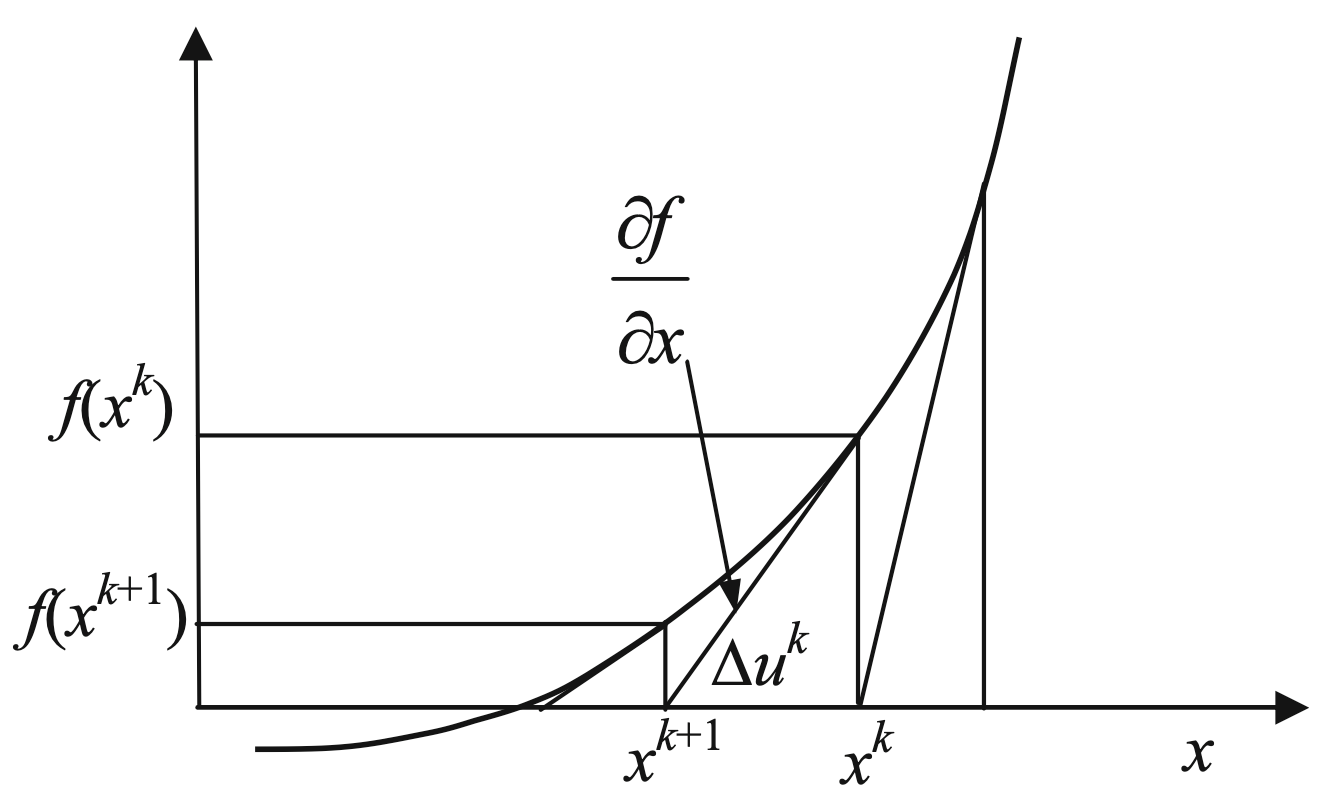
\includegraphics[width=0.45\textwidth]{Imagens/NR.png}
	\caption{Método de Newton–Raphson method para equação não linear, $f=0$}
	\label{fig:NR}
\end{figure}


A equação não linear, Eq.~\eqref{eq:formabilinear} pode ser linearizada usando o mesmo procedimento da Eq.~\eqref{eq:MetodoNR}. Como a forma de carga na Eq.~\eqref{eq:operadorForca} é independente do deslocamento, não é necessário linearizá-la. A linearização da forma de energia na Eq.~\eqref{eq:operadorBilinear} pode ser expressa como:
\begin{equation}\label{eq:LBilinear}
	L[a(\mathbf{u},\mathbf{\bar{u}})] = \iint_{\Omega_0} \Delta \mathbf{S} : \mathbf{\bar{E}} + \mathbf{S} : \Delta \mathbf{\bar{E}} , d\Omega,
\end{equation}
onde $\Delta \mathbf{S}$ é o incremento de tensão e $\Delta \mathbf{\bar{E}}$ é o incremento da variação de deformação. Para o material de St. Venant–Kirchhoff, a relação tensão-deformação é linear, e assim o incremento de tensão pode ser escrito como:
\begin{equation}
	\Delta \mathbf{S} = \frac{\partial \mathbf{S}}{\partial \mathbf{E}} : \Delta \mathbf{E} = \mathbf{D} : \Delta \mathbf{E},
\end{equation}
onde $\mathbf{D}$ é o tensor constitutivo de quarta ordem, e $\Delta \mathbf{E}$ é o incremento da deformação Lagrangiana. Observando que o incremento do gradiente de deformação é $\Delta \mathbf{F} = \nabla_0 \Delta \mathbf{u}$ da Eq.XXX {\color{red} falta uma parte sobre deformações e suas medidas e tensões e suas medidas}, o incremento da deformação Lagrangiana e sua variação podem ser obtidos como:
\begin{equation}
	\Delta \mathbf{E}(\mathbf{u}, \Delta \mathbf{u}) = \text{sym}(\nabla_0 \Delta \mathbf{u}^T \mathbf{F}),
\end{equation}
e
\begin{equation}
	\Delta \mathbf{\bar{E}}(\Delta \mathbf{u}, \mathbf{\bar{u}}) = \text{sym}(\nabla_0 \mathbf{\bar{u}}^T \nabla_0 \Delta \mathbf{u}).
\end{equation}

Assim, a linearização da forma de energia na Eq.~\eqref{eq:LBilinear} pode ser derivada em relação ao deslocamento e sua variação como:
\begin{equation}\label{eq:LBilinearFinal}
	L[a(\mathbf{u},\mathbf{\bar{u}})] = \iint_{\Omega_0} \mathbf{\bar{E}} : \mathbf{D} : \Delta \mathbf{E} + \mathbf{S} : \Delta \mathbf{\bar{E}}  d\Omega = a^*(\mathbf{u}; \Delta \mathbf{u}, \mathbf{\bar{u}}).
\end{equation}

A notação $a^*(\mathbf{u}; \Delta \mathbf{u}, \mathbf{\bar{u}})$ é usada para indicar que a forma depende implicitamente do deslocamento total $\mathbf{u}$ e é bilinear em relação a $\Delta u$ e $\mathbf{\bar{u}}$. O primeiro integrando de $a^*(\mathbf{u}; \Delta \mathbf{u}, \mathbf{\bar{u}})$ na Eq.~\eqref{eq:LBilinearFinal} depende da relação tensão-deformação e é chamado de \emph{rigidez tangente}, semelhante ao termo de rigidez em sistemas lineares. O segundo integrando, contendo o termo de tensão, só aparece em problemas não lineares geométricos e é chamado de \emph{rigidez inicial de tensão}.

Seja o passo de carga atual $t_n$ e o contador de iteração atual $k$. Assumindo que as cargas aplicadas são independentes do deslocamento, a equação incremental linearizada da Eq.~\eqref{eq:formabilinear} é obtida como:

\begin{equation}\label{eq:incrementolinearizado}
	a \left( u^n_k; \Delta u^k, u \right) = \ell \left( u \right) - a \left( u^n_k; u \right), \quad \forall u \in \mathbb{Z}; 
\end{equation}

e o deslocamento total é atualizado usando

\begin{equation}
	u^{n}_{k+1} = u^{n}_{k} + \Delta u^k. \tag{3.76}
\end{equation}

Observe que a equação incremental, Eq.~\eqref{eq:incrementolinearizado}, está na forma de $[K^n_k] \cdot \{ \Delta u^k \} = \{ R^n_k \}$ após discretização usando elementos finitos, o que será discutido na {\color{red}Seção XXXXX}. A Eq.~\eqref{eq:incrementolinearizado} é resolvida iterativamente até que o resíduo se anule, o que significa que a equação não linear original, Eq.~\eqref{eq:formabilinear}, é satisfe